% Progress report for the supervisor: gamma-CsPbI3 iodine vacancies
% Build: pdflatex presentation.tex (run twice). Figures are read from ../assets/.
\documentclass[aspectratio=169,10pt]{beamer}
\usetheme[progressbar=frametitle,numbering=fraction]{metropolis}
\usepackage[utf8]{inputenc}
\usepackage[T1]{fontenc}
\usepackage{lmodern}   % vector fonts (sharp text)
\usepackage{booktabs}
\usepackage{graphicx}
\usepackage{xcolor}
\graphicspath{{../assets/}}

\definecolor{pb}{HTML}{7F77DD}
\definecolor{iod}{HTML}{D85A30}
\definecolor{cs}{HTML}{1D9E75}
\setbeamercolor{alerted text}{fg=iod}

% ---------- Tsinghua colours (Tsinghua purple #660874) ----------
\definecolor{thupurple}{HTML}{660874}
\definecolor{thulight}{HTML}{F3E8F5}
\setbeamercolor{palette primary}{bg=thupurple, fg=white}
\setbeamercolor{frametitle}{bg=thupurple, fg=white}
\setbeamercolor{progress bar}{fg=thupurple!55, bg=thulight}
\setbeamercolor{progress bar in head/foot}{fg=thupurple!55, bg=thulight}
\setbeamercolor{progress bar in section page}{fg=thupurple, bg=thulight}
\setbeamercolor{title separator}{fg=thupurple}
\setbeamercolor{title}{fg=thupurple}
\setbeamercolor{section title}{fg=thupurple}
\setbeamercolor{structure}{fg=thupurple}
\setbeamercolor{itemize item}{fg=thupurple}
\setbeamercolor{itemize subitem}{fg=thupurple!70}
\setbeamercolor{enumerate item}{fg=thupurple}
\setbeamercolor{block title}{bg=thupurple, fg=white}
\setbeamercolor{block body}{bg=thulight, fg=black}
\setbeamercolor{block title alerted}{bg=iod, fg=white}
\setbeamercolor{block body alerted}{bg=iod!10, fg=black}
\setbeamercolor{footline}{fg=thupurple!80}
\setbeamercolor{normal text}{fg=black!85, bg=white}
\setbeamertemplate{footline}{%
  \begin{beamercolorbox}[wd=\paperwidth,ht=2.6ex,dp=1.2ex,leftskip=0.6cm,rightskip=0.6cm]{footline}%
    \usebeamerfont{page number in head/foot}%
    Duy M. Dao \quad$\vert$\quad Tsinghua University\hfill\insertframenumber/\inserttotalframenumber
  \end{beamercolorbox}}
\newcommand{\cpi}{$\gamma$-CsPbI$_3$}
\newcommand{\done}{\textcolor{cs}{\textbf{done}}}
\newcommand{\run}{\textcolor{iod}{\textbf{running}}}
\newcommand{\nxt}{\textcolor{gray}{next}}
\renewcommand{\arraystretch}{1.15}

% ---------- references: [n] marks in text, full entries at the foot of each slide ----------
\newcommand{\cit}[1]{\textsuperscript{\textcolor{gray}{[#1]}}}
\newcommand{\refs}[1]{\par\vfill\begingroup\tiny\color{gray}\raggedright #1\par\endgroup}
\newcommand{\RA}{[1] A.\,N.~Arber, Vikram, F.\,C.~Mocanu, M.\,S.~Islam, Chem.\ Mater.\ \textbf{37}, 4416 (2025).}
\newcommand{\RB}{[2] R.-I.~Biega, L.~Leppert, J.\ Phys.: Energy \textbf{3}, 034017 (2021).}
\newcommand{\RC}{[3] B.~Ahmad, M.\,S.\,R.~Limon, Z.~Ahmad, Phys.\ Rev.\ Mater.\ \textbf{8}, 125402 (2024).}
\newcommand{\RD}{[4] R.\,J.~Sutton \emph{et al.}, ACS Energy Lett.\ \textbf{3}, 1787 (2018).}
\newcommand{\RE}{[5] J.~Kaczkowski, I.~P{\l}owa\'s-Korus, J.\ Phys.\ Chem.\ Lett.\ \textbf{12}, 6613 (2021).}
\newcommand{\RF}{[6] A.~Seidu \emph{et al.}, J.\ Chem.\ Phys.\ \textbf{154}, 074712 (2021).}
\newcommand{\RI}{[7] J.\,P.~Perdew \emph{et al.}, Phys.\ Rev.\ Lett.\ \textbf{100}, 136406 (2008).}
\newcommand{\RJ}{[8] P.~Giannozzi \emph{et al.}, J.\ Phys.: Condens.\ Matter \textbf{21}, 395502 (2009); \textbf{29}, 465901 (2017).}
\newcommand{\RK}{[9] G.~Prandini \emph{et al.}, npj Comput.\ Mater.\ \textbf{4}, 72 (2018).}
\newcommand{\RL}{[10] J.~Even \emph{et al.}, J.\ Phys.\ Chem.\ Lett.\ \textbf{4}, 2999 (2013).}
\newcommand{\RM}{[11] C.~Freysoldt \emph{et al.}, Rev.\ Mod.\ Phys.\ \textbf{86}, 253 (2014).}
\newcommand{\RN}{[12] A.\,J.~Cohen, P.~Mori-S\'anchez, W.~Yang, Science \textbf{321}, 792 (2008).}
\newcommand{\RO}{[13] G.~Henkelman, B.\,P.~Uberuaga, H.~J\'onsson, J.\ Chem.\ Phys.\ \textbf{113}, 9901 (2000).}
\newcommand{\RP}{[14] S.~Smidstrup \emph{et al.}, J.\ Chem.\ Phys.\ \textbf{140}, 214106 (2014).}
\newcommand{\RQ}{[15] A.~Togo, K.~Shinohara, I.~Tanaka, Sci.\ Technol.\ Adv.\ Mater.: Methods \textbf{4}, 2384822 (2024).}
\newcommand{\RR}{[16] A.\,H.~Larsen \emph{et al.}, J.\ Phys.: Condens.\ Matter \textbf{29}, 273002 (2017).}
\newcommand{\RT}{[18] J.~Zhang \emph{et al.}, Appl.\ Surf.\ Sci.\ \textbf{679}, 161235 (2025).}
\newcommand{\RS}{[17] Y.~Huang, W.-J.~Yin, Y.~He, J.\ Phys.\ Chem.\ C \textbf{122}, 1345 (2018).}

\title{Iodine Vacancy Sites and Migration Paths in Bulk \cpi}
\subtitle{Progress report}
\author{Duy M. Dao}
\institute{School of Materials Science and Engineering, Tsinghua University}
\setbeamertemplate{title separator}{{\color{thupurple}\rule{\linewidth}{1.5pt}}\par\vspace{0.3em}}
\date{October 2026}

\begin{document}

\maketitle

% ---------------------------------------------------------------------
\begin{frame}{Goal and starting point}
  \small
  \textbf{Goal:} iodine-vacancy migration barriers in \cpi, hop by hop in the bulk \alert{(this talk)}, then layer by layer below the CsI-terminated (001) surface (later).
  Two iodine sites: apical \textbf{4c} (CsI layers) and equatorial \textbf{8d} (PbI$_2$ layers).

  \vspace{0.4em}
  \scriptsize
  \begin{tabular}{p{0.17\textwidth}p{0.42\textwidth}p{0.33\textwidth}}
    \toprule
    Paper & What it did & What it leaves open \\
    \midrule
    \textbf{A} Arber 2025\cit{1} & Bulk \cpi, PBEsol, 2$\times$2$\times$2: 0.34 eV (8d--8d), 0.35 eV (8d--4c), 0.77 eV (4c--4c) & One barrier per path \emph{type}; charge state not stated \\
    \textbf{B} Biega 2021\cit{2} & Cubic CsPbBr$_3$ slabs: long axial jump about halved at the surface & Long jump only; no tilt; slab never returns to bulk \\
    \textbf{C} Ahmad 2024\cit{3} & CsPbI$_3$ slab: vacancy formation energies vs depth & No barriers; slab middle off from its own bulk \\
    \textbf{D} Zhang 2025\cit{18} & Bulk \cpi\ under strain, PBEsol: two paths, 0.51 and 0.54 eV & Charge state; site energies; two paths only \\
    \bottomrule
  \end{tabular}

  \vspace{0.4em}
  \small
  \textbf{This talk:} \textbf{RQ1} Which site does the vacancy prefer, in each charge state? \quad
  \textbf{RQ2} Bulk barriers, and how the number and direction of hops shape transport?
  \refs{\RA\quad \RB\quad \RC\quad \RT}
\end{frame}

% ---------------------------------------------------------------------
\begin{frame}{Workflow}
  \footnotesize
  \begin{tabular}{clll}
    \toprule
    Step & Calculation & Purpose & Status \\
    \midrule
    1 & Unit cell: convergence, tight relaxation & Reference lattice & \done \\
    2 & Perfect 2$\times$2$\times$2 supercell (160 atoms) & Energy reference & \done \\
    3 & 4c and 8d vacancy, $+1$ and 0 & Site preference (RQ1) & 3/4 \done, 1 finishing \\
    4a & NEB stage 1: \textbf{S1, S2, L3, S6} & Hops with published values & inputs ready, \nxt \\
    4b & NEB stage 2: S3--S5 (L1, L2, L4 if needed) & Spread; hop network & \nxt \\
    5--7 & CsI-terminated (001) slab & Energies, barriers vs depth & later \\
    \bottomrule
  \end{tabular}

  \vspace{0.8em}
  Steps 1--4 are the bulk reference that every slab result is compared against.
\end{frame}

% ---------------------------------------------------------------------
\begin{frame}{Settings and why}
  \footnotesize
  \begin{tabular}{lll}
    \toprule
    Choice & Value & Why \\
    \midrule
    Code & Quantum ESPRESSO 6.5\cit{8} & One version for all production runs \\
    Functional & PBEsol\cit{7} & Good solid-state lattices; \textbf{same as paper A}\cit{1} \\
    SOC, dispersion & Not included & As paper A; SOC mainly shifts the Pb-$p$ band\cit{10} \\
    Pseudopotentials & SSSP 1.3 PBEsol efficiency\cit{9} & Verified library \\
    Cutoff & 60 Ry & 0.86 meV/atom from 80 Ry \\
    $k$-mesh & 4$\times$4$\times$3; supercell 2$\times$2$\times$2 & 0.23 meV/atom from 6$\times$6$\times$4 \\
    Forces & largest $< 0.01$ eV/\AA & Same as paper A \\
    Unit cell & tight relaxation & Soft result still drifted 0.2--0.3\% in $a$, $b$ \\
    \bottomrule
  \end{tabular}

  \vspace{0.5em}
  Relaxed cell 8.362 / 8.961 / 12.350 \AA\ (experiment\cit{4}: 8.577 / 8.856 / 12.472). Perfect supercell built from it needed \textbf{no relaxation} $\Rightarrow$ meshes consistent.

  \vspace{0.3em}
  Guiding rule: \alert{match paper A where possible}, so differences in results are physics, not settings.
  \refs{\RA\quad \RD\quad \RI\quad \RJ\quad \RK\quad \RL\quad Convergence and relaxations: this work.}
\end{frame}

% ---------------------------------------------------------------------
\begin{frame}{Defect supercell: choices and why}
  \footnotesize
  \begin{tabular}{p{0.3\textwidth}p{0.62\textwidth}}
    \toprule
    Choice & Why \\
    \midrule
    2$\times$2$\times$2 supercell, 159 atoms & Same as paper A\cit{1}; vacancy and its images 17--25 \AA\ apart \\
    Cell fixed at the bulk lattice & One dilute defect in a host whose lattice it cannot change\cit{11} \\
    Charge $+1$ first & Closed shell; stable state of $V_\mathrm{I}$ over most of the gap\cit{3,17} \\
    Neutral as well, spin-polarised & One extra electron; tests which charge state paper A used \\
    $k$-mesh kept at 2$\times$2$\times$2 & 2$\times$2$\times$1 test: forces 4$\times$ larger, 1.8 meV/atom shift $\rightarrow$ rejected \\
    No charge correction (yet) & Cancels in site differences and barriers (same charge at both ends)\cit{11} \\
    \bottomrule
  \end{tabular}
  \refs{\RA\quad \RC\quad \RM\quad \RS\quad $k$-mesh test: this work.}
\end{frame}

% ---------------------------------------------------------------------
\begin{frame}{RQ1: site preference depends on the charge state}
  \centering\small
  \begin{tabular}{lccc}
    \toprule
    & $E$(4c) (Ry) & $E$(8d) (Ry) & $\Delta E = E(\mathrm{8d}) - E(\mathrm{4c})$ \\
    \midrule
    $V_\mathrm{I}^{+1}$ & $-64954.16973158$ & $-64954.16980915$ & $\mathbf{-1}$ \textbf{meV} \\
    $V_\mathrm{I}^{0}$ & $-64953.80107772^{*}$ & $-64953.79815909$ & $\mathbf{\approx +40}$ \textbf{meV}$^{*}$ \\
    \midrule
    Paper A\cit{1}$^{\dagger}$ & & & $\approx -30$ meV \\
    Zhang 2025\cit{18}$^{\ddagger}$ & & & $\approx +15$ meV \\
    \bottomrule
  \end{tabular}

  {\scriptsize $^{*}$ Neutral 4c: forces converged, energy still settling ($\sim$0.4 meV/step).\quad $^{\dagger}$ From Fig.~S1; $^{\ddagger}$ from Fig.~6c; charge states not stated.}

  \vspace{0.4em}
  \raggedright\small
  \begin{itemize}
    \item $+1$: the two sites are \textbf{degenerate}.
    \item Neutral: \textbf{apical favoured} by $\approx$40 meV ($\approx$1.5\,$k_BT$ at 300 K $\Rightarrow$ $\sim$70\% of vacancies on 4c).
    \item Opposite in sign to paper A; same direction as the other PBEsol study.
  \end{itemize}
  \refs{\RA\ Not reported as a site energy; inferred from the end points of its Fig.~S1 ($\pm$0.01 eV).\quad \RT\quad Our energies: this work.}
\end{frame}

% ---------------------------------------------------------------------
\begin{frame}{The neutral vacancy is a shallow donor (in PBEsol)}
  \small
  \begin{tabular}{lll}
    \toprule
    Check & Result & Meaning \\
    \midrule
    Magnetisation of the neutral cells & 0.00\,$\mu_B$ throughout & extra electron not localised \\
    Fermi level $-$ pristine VBM & 1.56 eV (4c), 1.68 eV (8d) & at the conduction-band edge \\
    $\varepsilon(+/0) \approx E(0) - E(+1) - E_\mathrm{VBM}$ & 1.61 eV (4c), 1.65 eV (8d) & band gap $\approx$ 1.6 eV\cit{1} \\
    \bottomrule
  \end{tabular}

  \vspace{0.4em}
  Consistent with other work: PBEsol\cit{18}, PBE\cit{17}.

  \vspace{0.4em}
  \begin{alertblock}{Caveats}
    Rough numbers: no potential alignment or charge correction yet; gap taken from paper A. PBEsol tends to over-delocalise electrons\cit{12}; a hybrid-functional check would settle it.
  \end{alertblock}

  \footnotesize Consequence: in most conditions the vacancy is \textbf{+1}, where the two sites are degenerate $\Rightarrow$ NEB starts with $+1$.
  \refs{\RA\quad \RN\quad \RS\quad \RT\quad Our values: this work.}
\end{frame}

% ---------------------------------------------------------------------
\begin{frame}{Why do we disagree with paper A? The relaxed lattice}
  \centering\footnotesize
  \renewcommand{\arraystretch}{1.0}
  \begin{tabular}{llccc}
    \toprule
    Source & Method & Short / long in-plane axis (\AA) & $c$ (\AA) & In-plane difference \\
    \midrule
    Experiment, 293 K\cit{4} & X-ray & 8.577 / 8.856 & 12.47 & 3.3\% \\
    Kaczkowski 2021\cit{5} & LDA & 7.947 / 8.939 & 12.22 & 12.5\% \\
    \textbf{This work} & \textbf{PBEsol} & \textbf{8.362 / 8.961} & \textbf{12.35} & \textbf{7.2\%} \\
    Zhang 2025\cit{18} & PBEsol & 8.39 / 8.96 & 12.37 & 6.8\% \\
    Zhang 2025\cit{18} & HSE06 & 8.40 / 9.03 & 12.59 & 7.5\% \\
    Seidu 2021\cit{6} & PBEsol & 8.31 / 8.94 & 12.35 & 7.6\% \\
    Kaczkowski 2021\cit{5} & SCAN & 8.522 / 9.018 & 12.52 & 5.8\% \\
    Kaczkowski 2021\cit{5} & PBE & 8.731 / 9.095 & 12.64 & 4.2\% \\
    \alert{Paper A}\cit{1} & \alert{PBEsol} & \alert{8.68 / 8.71} & \alert{12.44} & \alert{0.3\%} \\
    \bottomrule
  \end{tabular}

  \vspace{0.2em}
  \raggedright\footnotesize
  \begin{itemize}
    \item Every 0 K relaxation is clearly rectangular, \emph{including a hybrid functional}; ours matches two independent PBEsol cells.
    \item Paper A's cell is nearly square $\Rightarrow$ weaker tilt $\Rightarrow$ 4c and 8d more alike: may explain part of the disagreement.
  \end{itemize}
  \refs{\RA\quad \RD\quad \RE\quad \RF\ (converted from its rotated setting).\quad \RT\ (Table S1).}
\end{frame}

% ---------------------------------------------------------------------
\begin{frame}{RQ2: ten distinct hops, not three}
  \centering
  \vspace*{-0.8em}
  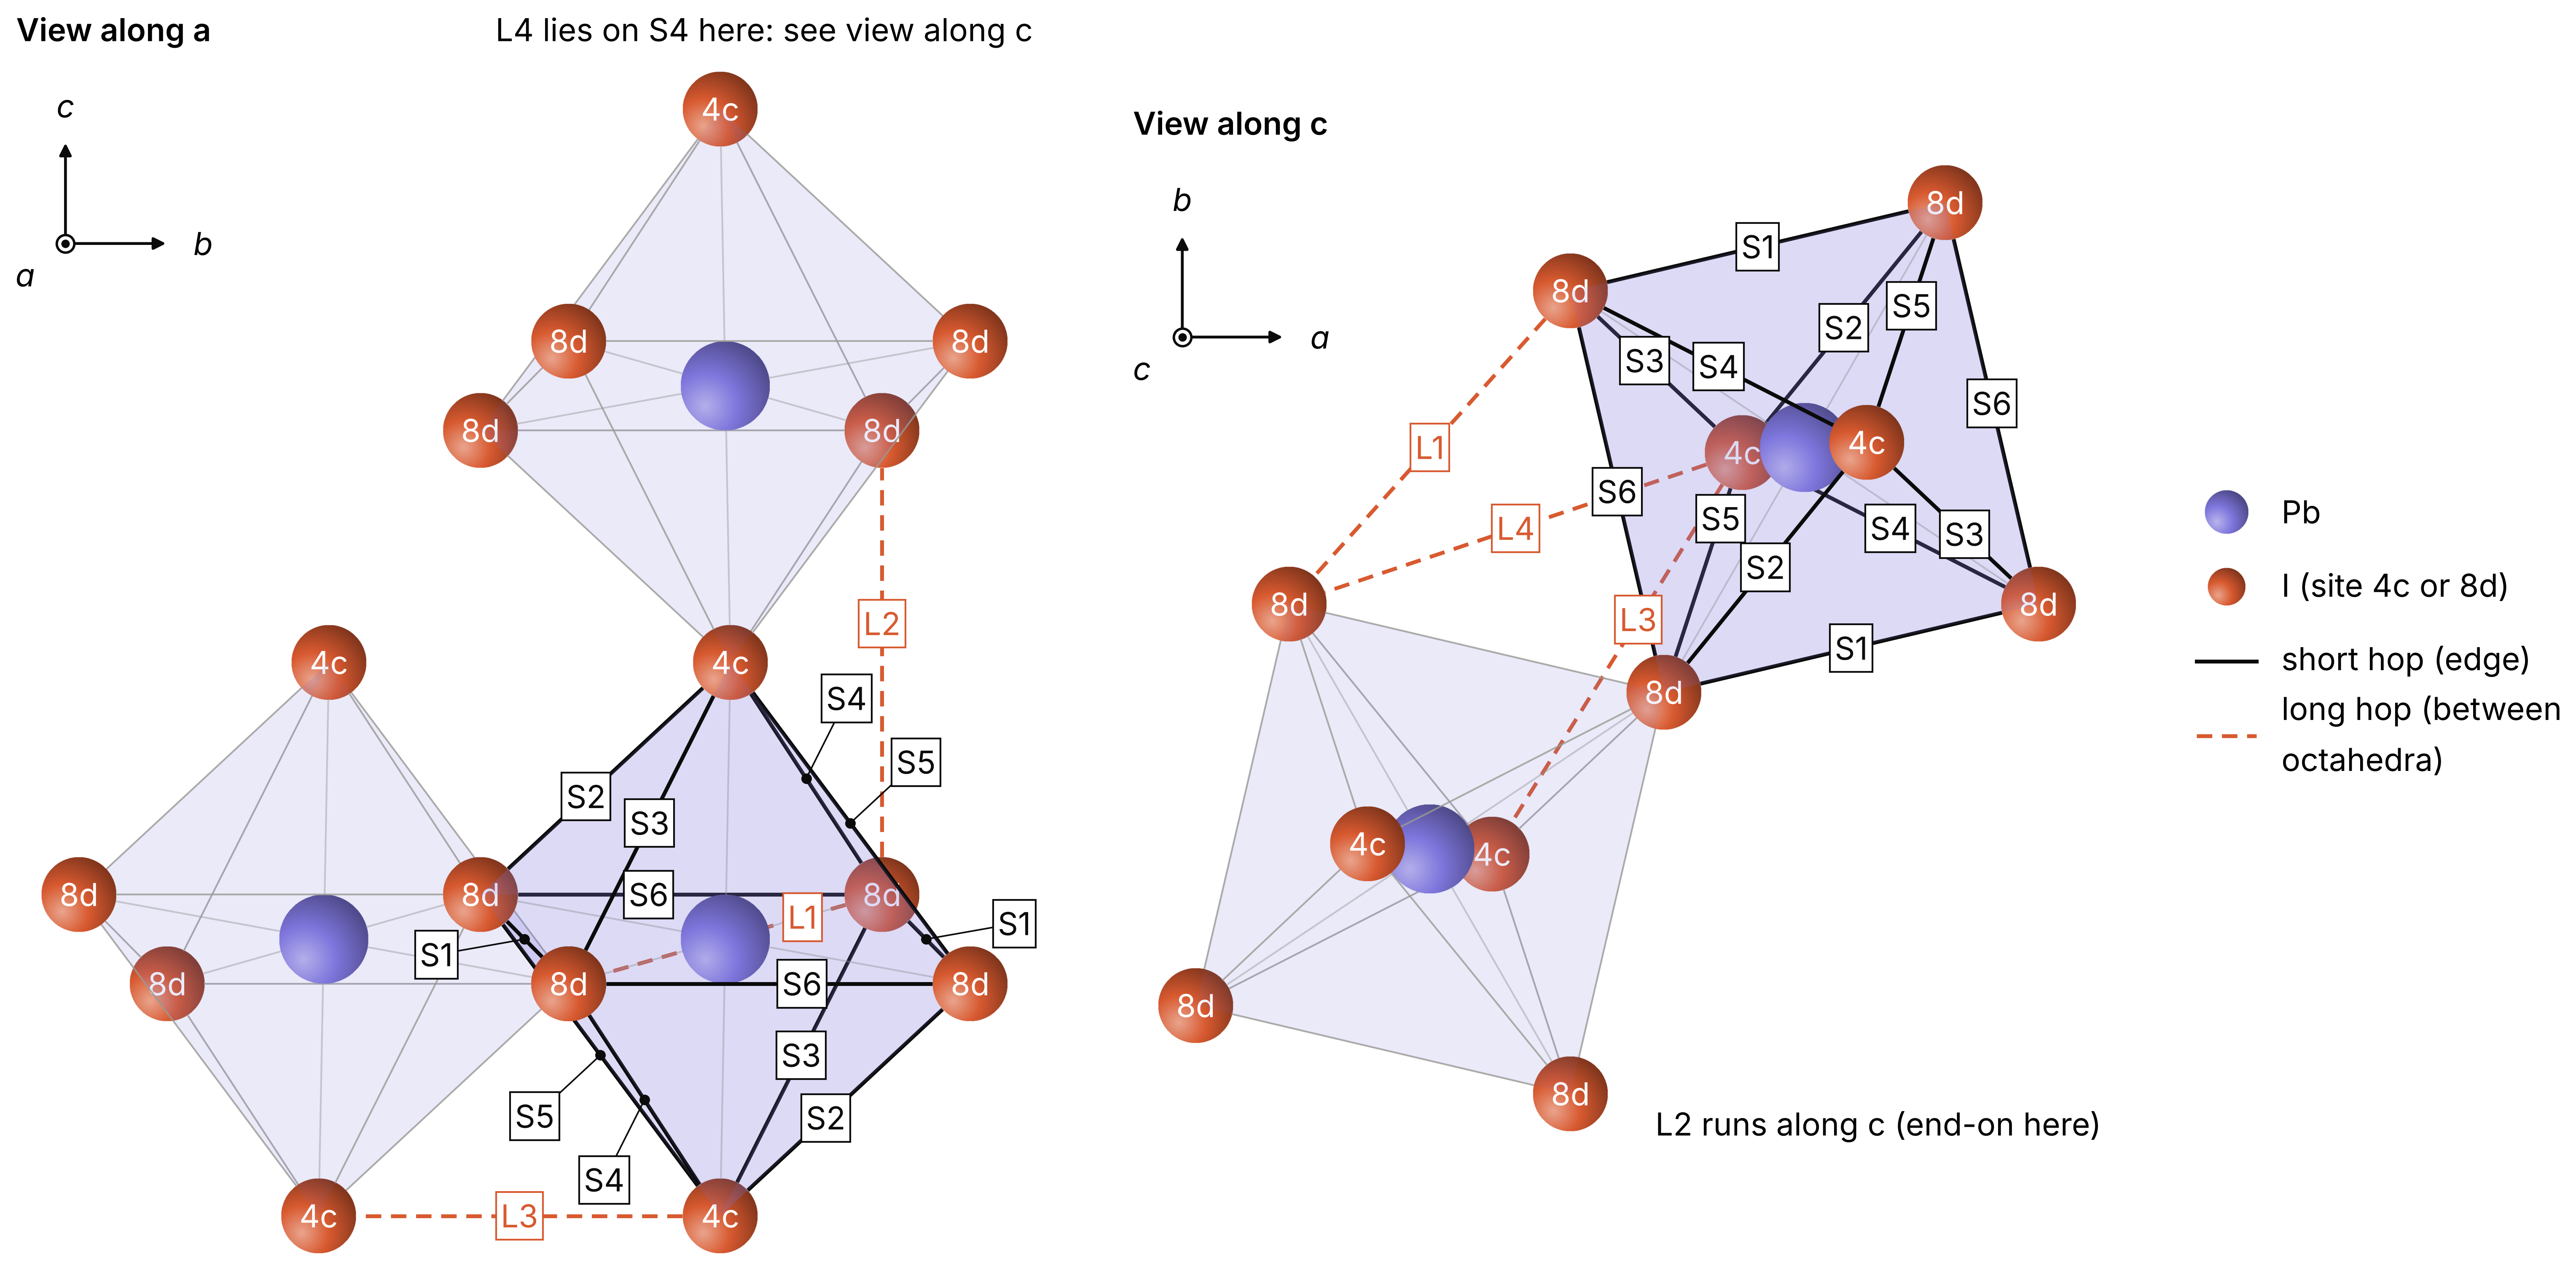
\includegraphics[width=\textwidth,height=0.83\textheight,keepaspectratio]{octahedra_hops_wide.png}
  \refs{S1--S6: along octahedron edges (Pb is an inversion centre: 12 edges $\rightarrow$ 6); L1--L4: between corner-sharing octahedra. This work.}
\end{frame}

% ---------------------------------------------------------------------
\begin{frame}{The hop network: how many, and where they go}
  \centering\footnotesize
  \begin{tabular}{llcccl}
    \toprule
    Hop & Ends & Length (\AA) & From 8d & From 4c & Moves the vacancy \\
    \midrule
    S1, S6 & 8d--8d & 4.41, 4.60 & 2 each & 0 & within a PbI$_2$ layer \\
    S2--S5 & 4c--8d & 4.43--4.56 & 1 each & 2 each & PbI$_2$ $\leftrightarrow$ CsI layer \\
    L1 & 8d--8d & 4.80 & 1 & 0 & within a PbI$_2$ layer \\
    L2 & 8d--8d & 5.18 & 1 & 0 & straight along $c$ \\
    L3 & 4c--4c & 5.28 & 0 & 2 & within a CsI layer \\
    L4 & 4c--8d & 5.93 & 1 & 2 & between layers \\
    \midrule
    Total & & & 11 & 12 & \\
    \bottomrule
  \end{tabular}

  \vspace{0.3em}
  \raggedright\footnotesize
  \begin{itemize}
    \item A 4c vacancy has \textbf{no short hop to another 4c}: every move starts 4c $\rightarrow$ 8d
    \item ab plane: 8d--8d hops suffice. Along $c$: \textbf{4c--8d hops} (8d$\rightarrow$4c$\rightarrow$8d) or the long L2
    \item Transport depends on barriers \emph{and} hop numbers \emph{and} site energies $\Rightarrow$ anisotropic diffusion
  \end{itemize}
  \refs{Counts and directions: this work (\texttt{hop\_network.py}). Paper A treats one barrier per type\cit{1}.\quad \RA}
\end{frame}

% ---------------------------------------------------------------------
\begin{frame}{NEB plan: start with hops that have published values}
  \scriptsize
  \begin{tabular}{llll}
    \toprule
    Published path & Value & Our hop & How identified \\
    \midrule
    Paper A: 4c--4c\cit{1} & 0.77 eV & \textbf{L3} & only 4c--4c hop \\
    Paper A: 8d--8d, 8d--4c\cit{1} & 0.34, 0.35 eV & S1/S6; one of S2--S5 & schematic only \\
    Zhang: in-plane\cit{18} & 0.54 eV & \textbf{S1} (probable) & rises $\approx$1 \AA\ along $c$ (S6: 0) \\
    Zhang: out-of-plane\cit{18} & 0.51 eV & \textbf{S2} (probable) & rises $\approx$2.7 \AA, no sideways shift \\
    \bottomrule
  \end{tabular}

  \vspace{0.3em}
  \begin{tabular}{clp{0.55\textwidth}}
    \toprule
    Stage & Hops & Purpose \\
    \midrule
    1 & S1, S2, L3, S6 & Compare with published values; S1 vs S6 = first spread within a type \\
    2 & S3, S4, S5 & Spread of the 4c--8d hops (control transport along $c$) \\
    3 & L1, L2, L4 & Only if the network analysis needs them \\
    \bottomrule
  \end{tabular}

  \vspace{0.3em}
  \textbf{Setup:} end points by symmetry from the relaxed vacancies (64 Pnma operations\cit{15}), IDPP path\cit{14,16}, climbing image\cit{13}, 4 images, $k$ 2$\times$2$\times$2; both directions reported. Spread $<$ 0.03 eV $\Rightarrow$ one barrier per type (0.05 eV $\approx 7\times$ in rate at 300 K).
  \refs{\RA\quad \RO\quad \RP\quad \RQ\quad \RR\quad \RT\ (paths assigned from its Fig.~6a,b, $\pm$0.3 \AA).}
\end{frame}

% ---------------------------------------------------------------------
\begin{frame}{Questions for discussion}
  \begin{enumerate}
    \item \textbf{Paper A's lattice:} rerun our $+1$ pair on their cell (8.68/8.71/12.44 \AA) to test the tilt explanation? About one week.
    \item \textbf{Shallow donor:} is a hybrid-functional check, or a proper $\varepsilon(+/0)$ with corrections, worth the cost?
    \item \textbf{Spin--orbit coupling:} single-point check on the site energies now, or after the barriers?
    \item \textbf{NEB scope:} start with the 4 hops with published values, then decide; neutral only for stage 1?
    \item Contact paper A's authors about their charge state and end-point energies?
  \end{enumerate}
\end{frame}

% ---------------------------------------------------------------------
\begin{frame}{Summary}
  \begin{itemize}
    \item \textbf{Bulk reference built:} converged settings, tight lattice, perfect and vacancy supercells.
    \item \textbf{Site preference depends on charge:} $+1$ degenerate; neutral favours 4c by $\approx$40 meV, opposite to paper A.
    \item \textbf{Neutral vacancy is a shallow donor} in PBEsol $\Rightarrow$ $+1$ is the relevant state.
    \item \textbf{Benchmark mismatch} likely from paper A's nearly square, less-tilted cell.
    \item \textbf{Ten hops}; transport along $c$ needs 4c--8d hops $\Rightarrow$ staged NEB, starting with S1, S2, L3, S6.
  \end{itemize}

  \vspace{1em}
  \centering
  \textbf{Next: NEB stage 1 at $+1$ against 0.34, 0.51, 0.54 and 0.77 eV.}
\end{frame}

\begin{frame}[allowframebreaks]{References}
  \tiny
  \begin{itemize}\setlength{\itemsep}{1pt}
    \item[] \RA
    \item[] \RB
    \item[] \RC
    \item[] \RD
    \item[] \RE
    \item[] \RF
    \item[] \RI
    \item[] \RJ
    \item[] \RK
    \item[] \RL
    \item[] \RM
    \item[] \RN
    \item[] \RO
    \item[] \RP
    \item[] \RQ
    \item[] \RR
    \item[] \RS
    \item[] \RT
  \end{itemize}
\end{frame}

\end{document}
